\newpage

\section{Interdependencia y ganancias derivadas del comercio} La interdependencia entre productores debe entenderse como una forma de producción mas eficiente, con una mayor variedad de productos disponibles para el consumidor. Por lo que se parte del comercio implica un aumento de la prosperidad y eficiencia entre las partes. 
\subsection{Importaciones} Productos producidos fuera del territorio nacional,en dondé se tiene una desventaja relativa o absoluta en la producción. 
\subsection{Exportaciones} Productos producidos fentro del territorio nacional, en dondé se tiene una ventaja absoluta o relativa.  
\subsection{Ventajas} Cuando un productor puede generar el mismo producto con una menor cantidad de factores se dice que tiene una ventaja absoluta,Ventaja relativa acorde a un productor que tiene un coste de oportunidad mas bajo.

\begin{figure}[h]
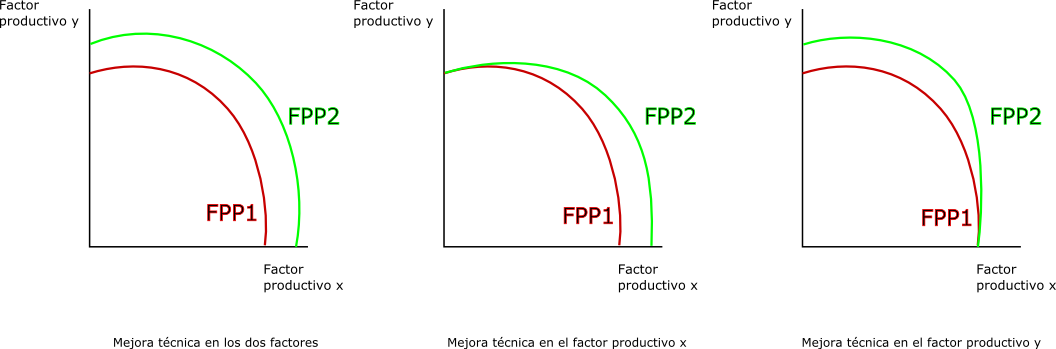
\includegraphics[scale=0.3]{images/Desplazamientos_en_la_FPP.png}
\end{figure}
Existen distintas formas de mejoras en los factores a producir, ya sea con mejoras en la forma productiva (Tecnología)de un bien o de ambos. en ambos casos se logra alcanzar puntos que antes era inalcanzables para el productor.

